% Drawing 148/01-4 -- folder 148, batch 01, archive page 14 (PDF page 15).
% Transcription: à gauche, un croquis : l'hexagone subdivisé en triangles, un losange de quatre petits triangles repassé en gras. Le « 12 » des arêtes surcharge un autre chiffre. Le reste de la page est blanc ; la suite paginée par lui s'arrête ici, à sa p.~6
% Kind: hexagon subdivided into triangles. Method 2 (schematic redraw from the facsimile). Status: partial.
% Notes: Hexagon L, TL, TR, R, BR, BL with its three diagonals through the centre O, and in the upper right the lattice of small triangles (edge 1/2 of the side): the lattice points are computed once as the midpoints of the half-diagonals and of the sides TL-TR and TR-R, and every stroke is drawn between them, so the lattice lines meet exactly there. Heavy strokes (all overdrawn on the page): seven small triangles of the upper right, the half-diagonal O-BR and the right half of the horizontal diagonal; thin: the rest of the outline, the left half of the horizontal diagonal, the half-diagonal O-BL, and the left half of the top side. Dots at the three lattice points he marked (middle of O-TL, O, middle of O-R). The heavy rhombus of four small triangles of the transcription is not singled out from the other heavy strokes. A short pencil stroke at the lower left (no head visible) is drawn; the "12" (in the text, overwriting another figure) and an ink blot under it are left out. Still differs: on the page the hexagon is wider on the left (the lattice is not regular), and the strokes are curved and overshoot; the lattice points are where the drawn lines cross, to within about 1.5 units. Redrawn 2026-11-09 (issue 128): to check again.
% Coordinates: 1 unit = 1 mm = 1/100 of the crop width (bbox in page fractions: [0.11, 0.38, 0.35, 0.5]).
% Redrawn by Claude (claude-opus-5-5), issue #73, 2026-11-09; not checked by a human; not compiled (no TeX in the session).
% Rights: reproduces part of the work -- behind RENDER_TRANSCRIPTS, never published by itself.
\documentclass[tikz,border=3pt]{standalone}
\usepackage{amsmath,amssymb}
\usetikzlibrary{patterns,arrows.meta}
\tikzset{pencil/.style={black!45}, struck/.style={black!35}, mark/.style={circle,draw,inner sep=1.3pt}, pt/.style={circle,fill,inner sep=0.9pt}, opt/.style={circle,draw,fill=white,inner sep=1.1pt}}
\begin{document}
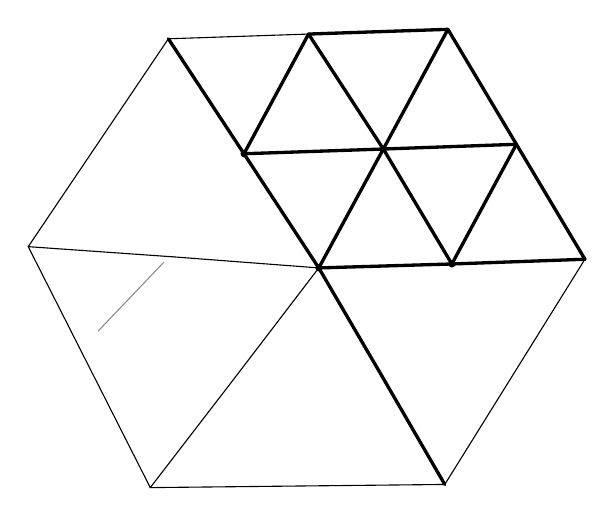
\begin{tikzpicture}[x=1mm,y=1mm,line cap=round,line join=round,font=\scriptsize]
\draw (38.2,-6.8) -- (56,-6.2);
\draw (20.4,-33.2) -- (38.2,-6.8);
\draw (20.4,-33.2) -- (38.9,-34.5);
\draw (38.9,-34.5) -- (57.3,-35.9);
\draw (57.3,-35.9) -- (46.6,-49.9);
\draw (46.6,-49.9) -- (35.9,-63.8);
\draw (35.9,-63.8) -- (73.3,-63.4);
\draw (91.1,-34.8) -- (73.3,-63.4);
\draw (20.4,-33.2) -- (35.9,-63.8);
\draw[very thick] (56,-6.2) -- (73.7,-5.6);
\draw[very thick] (38.2,-6.8) -- (47.8,-21.4);
\draw[very thick] (47.8,-21.4) -- (57.3,-35.9);
\draw[very thick] (56,-6.2) -- (47.8,-21.4);
\draw[very thick] (56,-6.2) -- (65.5,-20.8);
\draw[very thick] (47.8,-21.4) -- (65.5,-20.8);
\draw[very thick] (65.5,-20.8) -- (82.4,-20.2);
\draw[very thick] (73.7,-5.6) -- (65.5,-20.8);
\draw[very thick] (65.5,-20.8) -- (57.3,-35.9);
\draw[very thick] (73.7,-5.6) -- (82.4,-20.2);
\draw[very thick] (82.4,-20.2) -- (91.1,-34.8);
\draw[very thick] (65.5,-20.8) -- (74.2,-35.4);
\draw[very thick] (82.4,-20.2) -- (74.2,-35.4);
\draw[very thick] (57.3,-35.9) -- (74.2,-35.4);
\draw[very thick] (74.2,-35.4) -- (91.1,-34.8);
\draw[very thick] (57.3,-35.9) -- (65.3,-49.6);
\draw[very thick] (65.3,-49.6) -- (73.3,-63.4);
\node[pt] at (47.8,-21.4) {};
\node[pt] at (57.3,-35.9) {};
\node[pt] at (74.2,-35.4) {};
\draw[pencil] (29.3,-43.9) -- (37.6,-35.2);
\end{tikzpicture}
\end{document}
